
% POSTER EXAMPLE
%
% This is an example of a relatively sane poster. The box structure (and the
% narrative in general) is what I would expect, but it is completely
% non-mandatory; you may include whatever you want. Preferably, erase the
% existing box structure after you read it, and start from scratch.
%
% The main communication requirements for the poster that should be satisfied
% are as such:
%
% - At the defense, it should help you talk for around 10 minutes about your
%   thesis, and convince the committee that you did something interesting and
%   sufficiently complicated. Prepare pictures that explain your main results.
%
% - It should quickly communicate the main idea of your thesis to a random
%   educated by-walker. Ideally, a moderately-witted MFF graduate who has never
%   heard about your thesis before should be able to get the main "rough idea"
%   in less than 1 minute by just looking at the poster.

% modify the fontscale parameter to make everything slighly bigger or smaller.
\documentclass[portrait,a0paper,fontscale=0.25]{baposter}

\usepackage[utf8]{inputenc}
\usepackage[T1]{fontenc}

% FONT CHOICES
% Posters do not need to be PDF/A; you can choose any relatable font from the
% TeX font catalogue without much risk. Sans-serif fonts are suggested for the
% posters; see https://tug.org/FontCatalogue/sansseriffonts.html
\usepackage[sfdefault]{Fira Sans}
%\usepackage[default]{droidsans}
%\usepackage[math]{iwona}
%\usepackage[defaultfam]{montserrat}
%\usepackage{cmbright}
%\usepackage{yfonts}\renewcommand{\familydefault}{\frakdefault}

\usepackage{color}
\usepackage{graphicx}
\usepackage{amssymb,amsmath}
\usepackage[export]{adjustbox} %allows using valign with \includegraphics

\renewcommand{\arraystretch}{1.5}

\usetikzlibrary{positioning}

% A WORD ABOUT COLORS
%
% This template is prepared with a relatively neutral gray background that
% gives decent box borders (with white and darker gray), does not clash with
% many colors (except for violet-brown and other mushroomish colors, perhaps)
% and gives a lot of space for highlighting stuff.
%
% Generally, other color variations are good too; there are no strict rules on
% the colors. Good choices include:
%
% - white backgrounds and differentiation of box headers by color (see
%   headerFontColor)
%
% - various slightly tinted backgrounds (try red!10 instead of black!3)
% 
% - dark backgrounds
%
% Keep in mind:
% - The normal "informative" text and figures should be DARK on LIGHT
%   background, not the other way around.
%
% - If you want a dark background, soften (darken) the box backgrounds a bit so
%   that they do not "shine" too much from the poster. Use \color{white} for
%   the heading, and switch the UK/MFF logos to white (see contents of logos/).
%
% - Do not mix too many color hues together. Most hues have their widely
%   accepted meaning (green: good result, red: problem, blue: information,
%   yellow: highlighter, brown: serious problem, violet: something really
%   weird/interesting/magic, depending on the shade).

\begin{document}

\color{black!80} % default font color
\begin{poster}{grid=false,
	eyecatcher=true,
	background=plain,
	bgColorOne=black!3, % background color
	columns=2,
	headerborder=none,
	textborder=none,
	headershape=rectangle,
	headershade=plain,
	boxshade=plain,
	boxColorOne=white,
	headershade=plain,
	headerColorOne=black!15, % box header background color
	headerFontColor=black,
	}%
	{
\includegraphics[height=7em]{logos/mff-black.pdf}}
	{Extension of web-based interface for protein binding sites prediction}
	{\vspace{1ex} Lukáš Polák}
	{
\includegraphics[height=7em]{logos/uk-red.pdf}}


%
% LEFT COLUMN
%

\begin{posterbox}[column=0,name=intro]{Introduction}

Detection of protein ligand-binding sites is a vital aspect of nowadays drug discovery and development. Identification of the potential binding sites (also called pockets) allows an understanding of various molecule interactions, which is the first step of rational drug discovery pipelines.

PrankWeb is a web-based tool developed at MFF UK for visualizing predictions of protein binding sites. It is based on the P2Rank tool that predicts binding sites quickly and efficiently. The website is used by thousands of users every month.

%\begin{center}\begin{tikzpicture}[ultra thick, inner sep=1ex]
%\node[rectangle, rounded corners=1ex, draw=red!80!black, color=red!80!black, font=\huge\bfseries, rotate=21] {Problem!};
%\end{tikzpicture}\end{center}

\end{posterbox}

\begin{posterbox}[column=0, name=goals, below=intro, headerColorOne=cyan!60, boxColorOne=cyan!20]{Thesis goals}
There were two main goals of the thesis:
\begin{itemize}
\item Improve the web frontend and replace old and unsupported components with new ones.
\item Extend the server architecture to enable the simple addition of modules (plugins) for postprocessing of the predicted binding sites.
\end{itemize}
\end{posterbox}

\begin{posterbox}[column=0, name=architecture, below=goals]{Server architecture}

The architecture of PrankWeb is rather complex and consists of several components.
For simplicity, the architecture may be divided as follows:

\begin{center}
	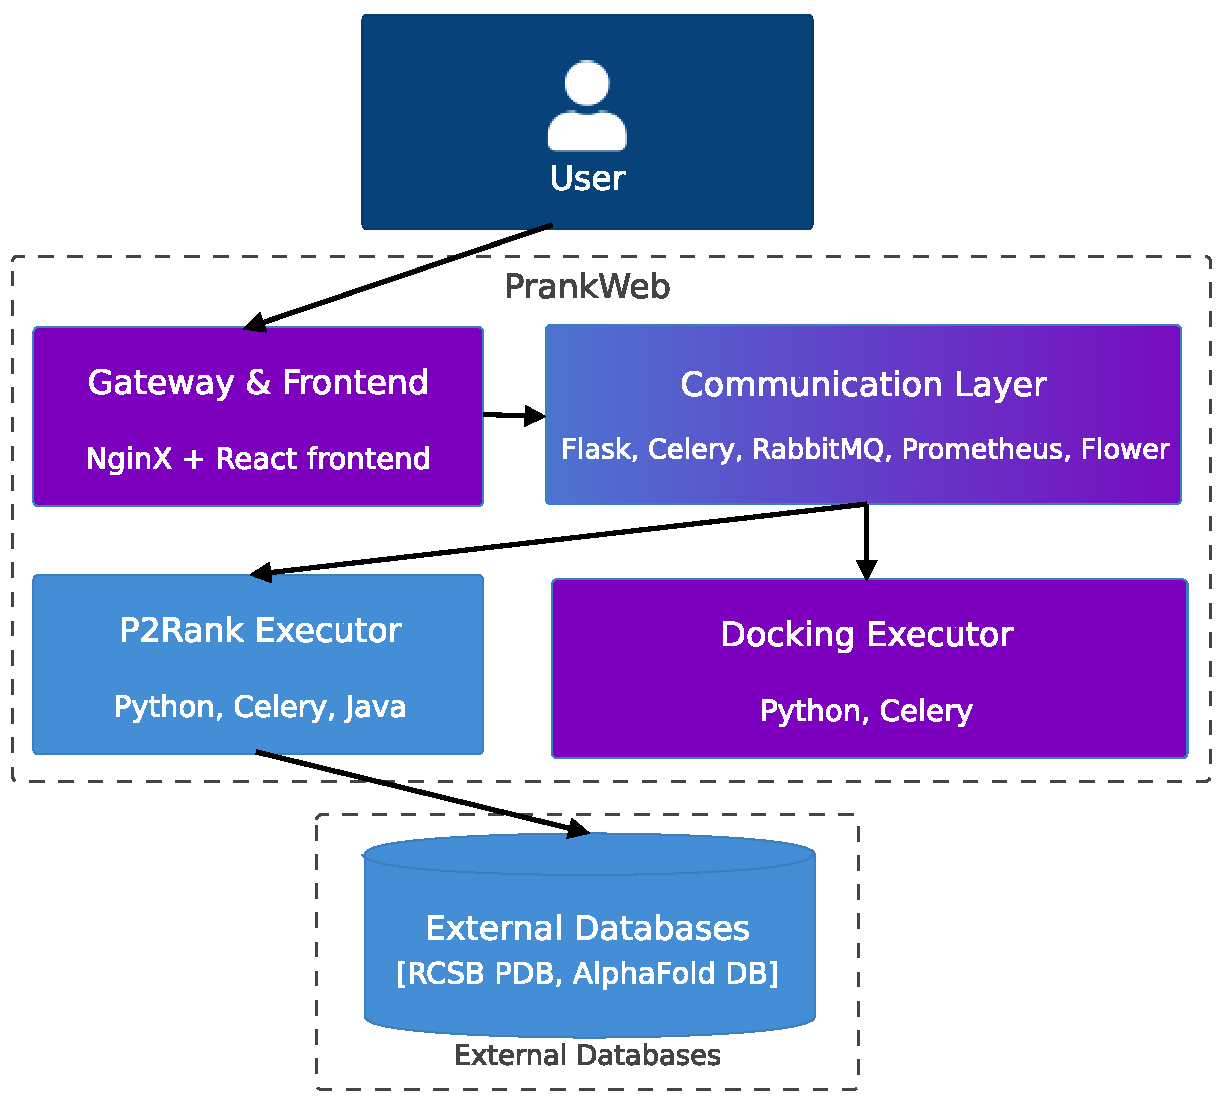
\includegraphics[width=0.8\linewidth]{img/arch.pdf}
\end{center}

The nodes of the diagram do not represent actual containers, but logical units of the system. Blue nodes represent units that were not modified during the thesis, purple nodes represent units that were substantially modified or added during the implementation.

%\tikzstyle{rec}=[rectangle, draw, rounded corners=1ex, font=\huge\bfseries]
%\begin{center}\begin{tikzpicture}[ultra thick, inner sep=1ex]
%\node[rec] (a) {Keep};
%\node[rec, circle, right=of a] (b) {it};
%\node[rec, right=of b] (c) {simple};
%\node[rec, densely dotted, below=6cm of c, font=\small] (notice) {\dots{}but precise!};
%\draw[->] (a) to (b);
%\draw[->] (b) to (c);
%\draw[dotted] (notice) to (c);
%\end{tikzpicture}\end{center}

\end{posterbox}

\begin{posterbox}[column=0, name=tech, below=architecture, headerColorOne=yellow!80!orange!95!black, boxColorOne=yellow!33]{Thesis-specific technologies}
\begin{itemize}
	\item \textbf{Frontend} - React (TypeScript), specialized open-source libraries Mol* and RCSB Saguaro 1D Viewer
	\item \textbf{Backend} - Python, Flask, Celery
\end{itemize}
The entire project is dockerized and deployed via Docker-compose. Some of the containers use different technologies as well (e.g. Java), but those were not affected by the thesis.
\end{posterbox}

%
% FOOTER
%

%\begin{posterbox}[column=0, span=2, name=footer, below=tech,
%	textborder=none, headerborder=none, boxheaderheight=0pt,
%	boxColorOne=black!3]{}
%If some institute/grant/department sponsored the work, put an acknowledgement here.
%\end{posterbox}

%
% RIGHT COLUMN
%
% It is usually best to fill most of the poster with your results and
% conclusions. Again, use simple annotated pictures wherever possible. Plots
% with measurements are perfect, tables are also good.
%

\begin{posterbox}[column=1, name=result1]{Frontend}
\begin{center}
	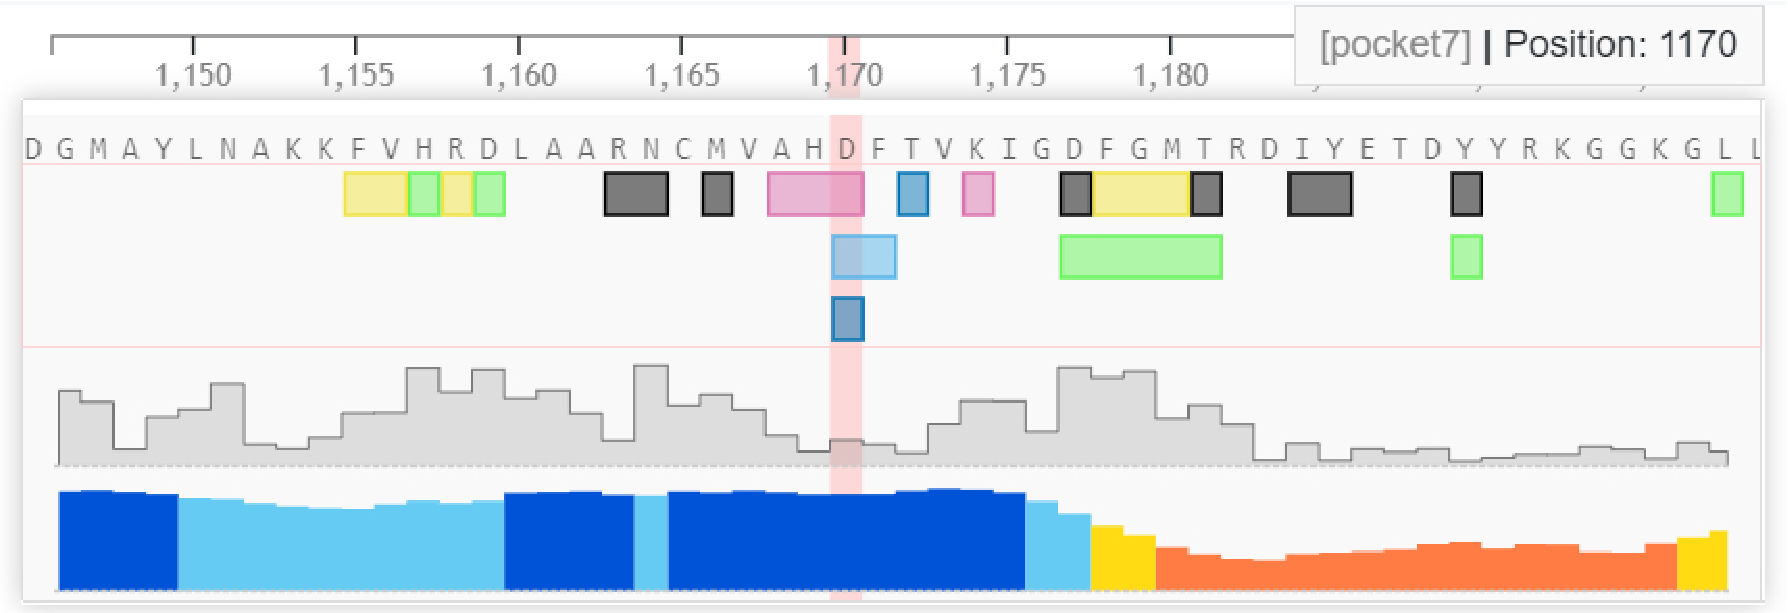
\includegraphics[width=0.8\linewidth]{img/1D.pdf}
\end{center}

One of the two replaced components is the 1D viewer. We employed the RCSB Saguaro 1D Viewer.
In the picture, the viewer shows the human insulin receptor protein sequence (UniProt ID P06213) with the predicted binding sites colored in the same theme as in Mol*.
The conservation and AlphaFold confidence scores are shown in the form of a histogram.

\begin{center}
	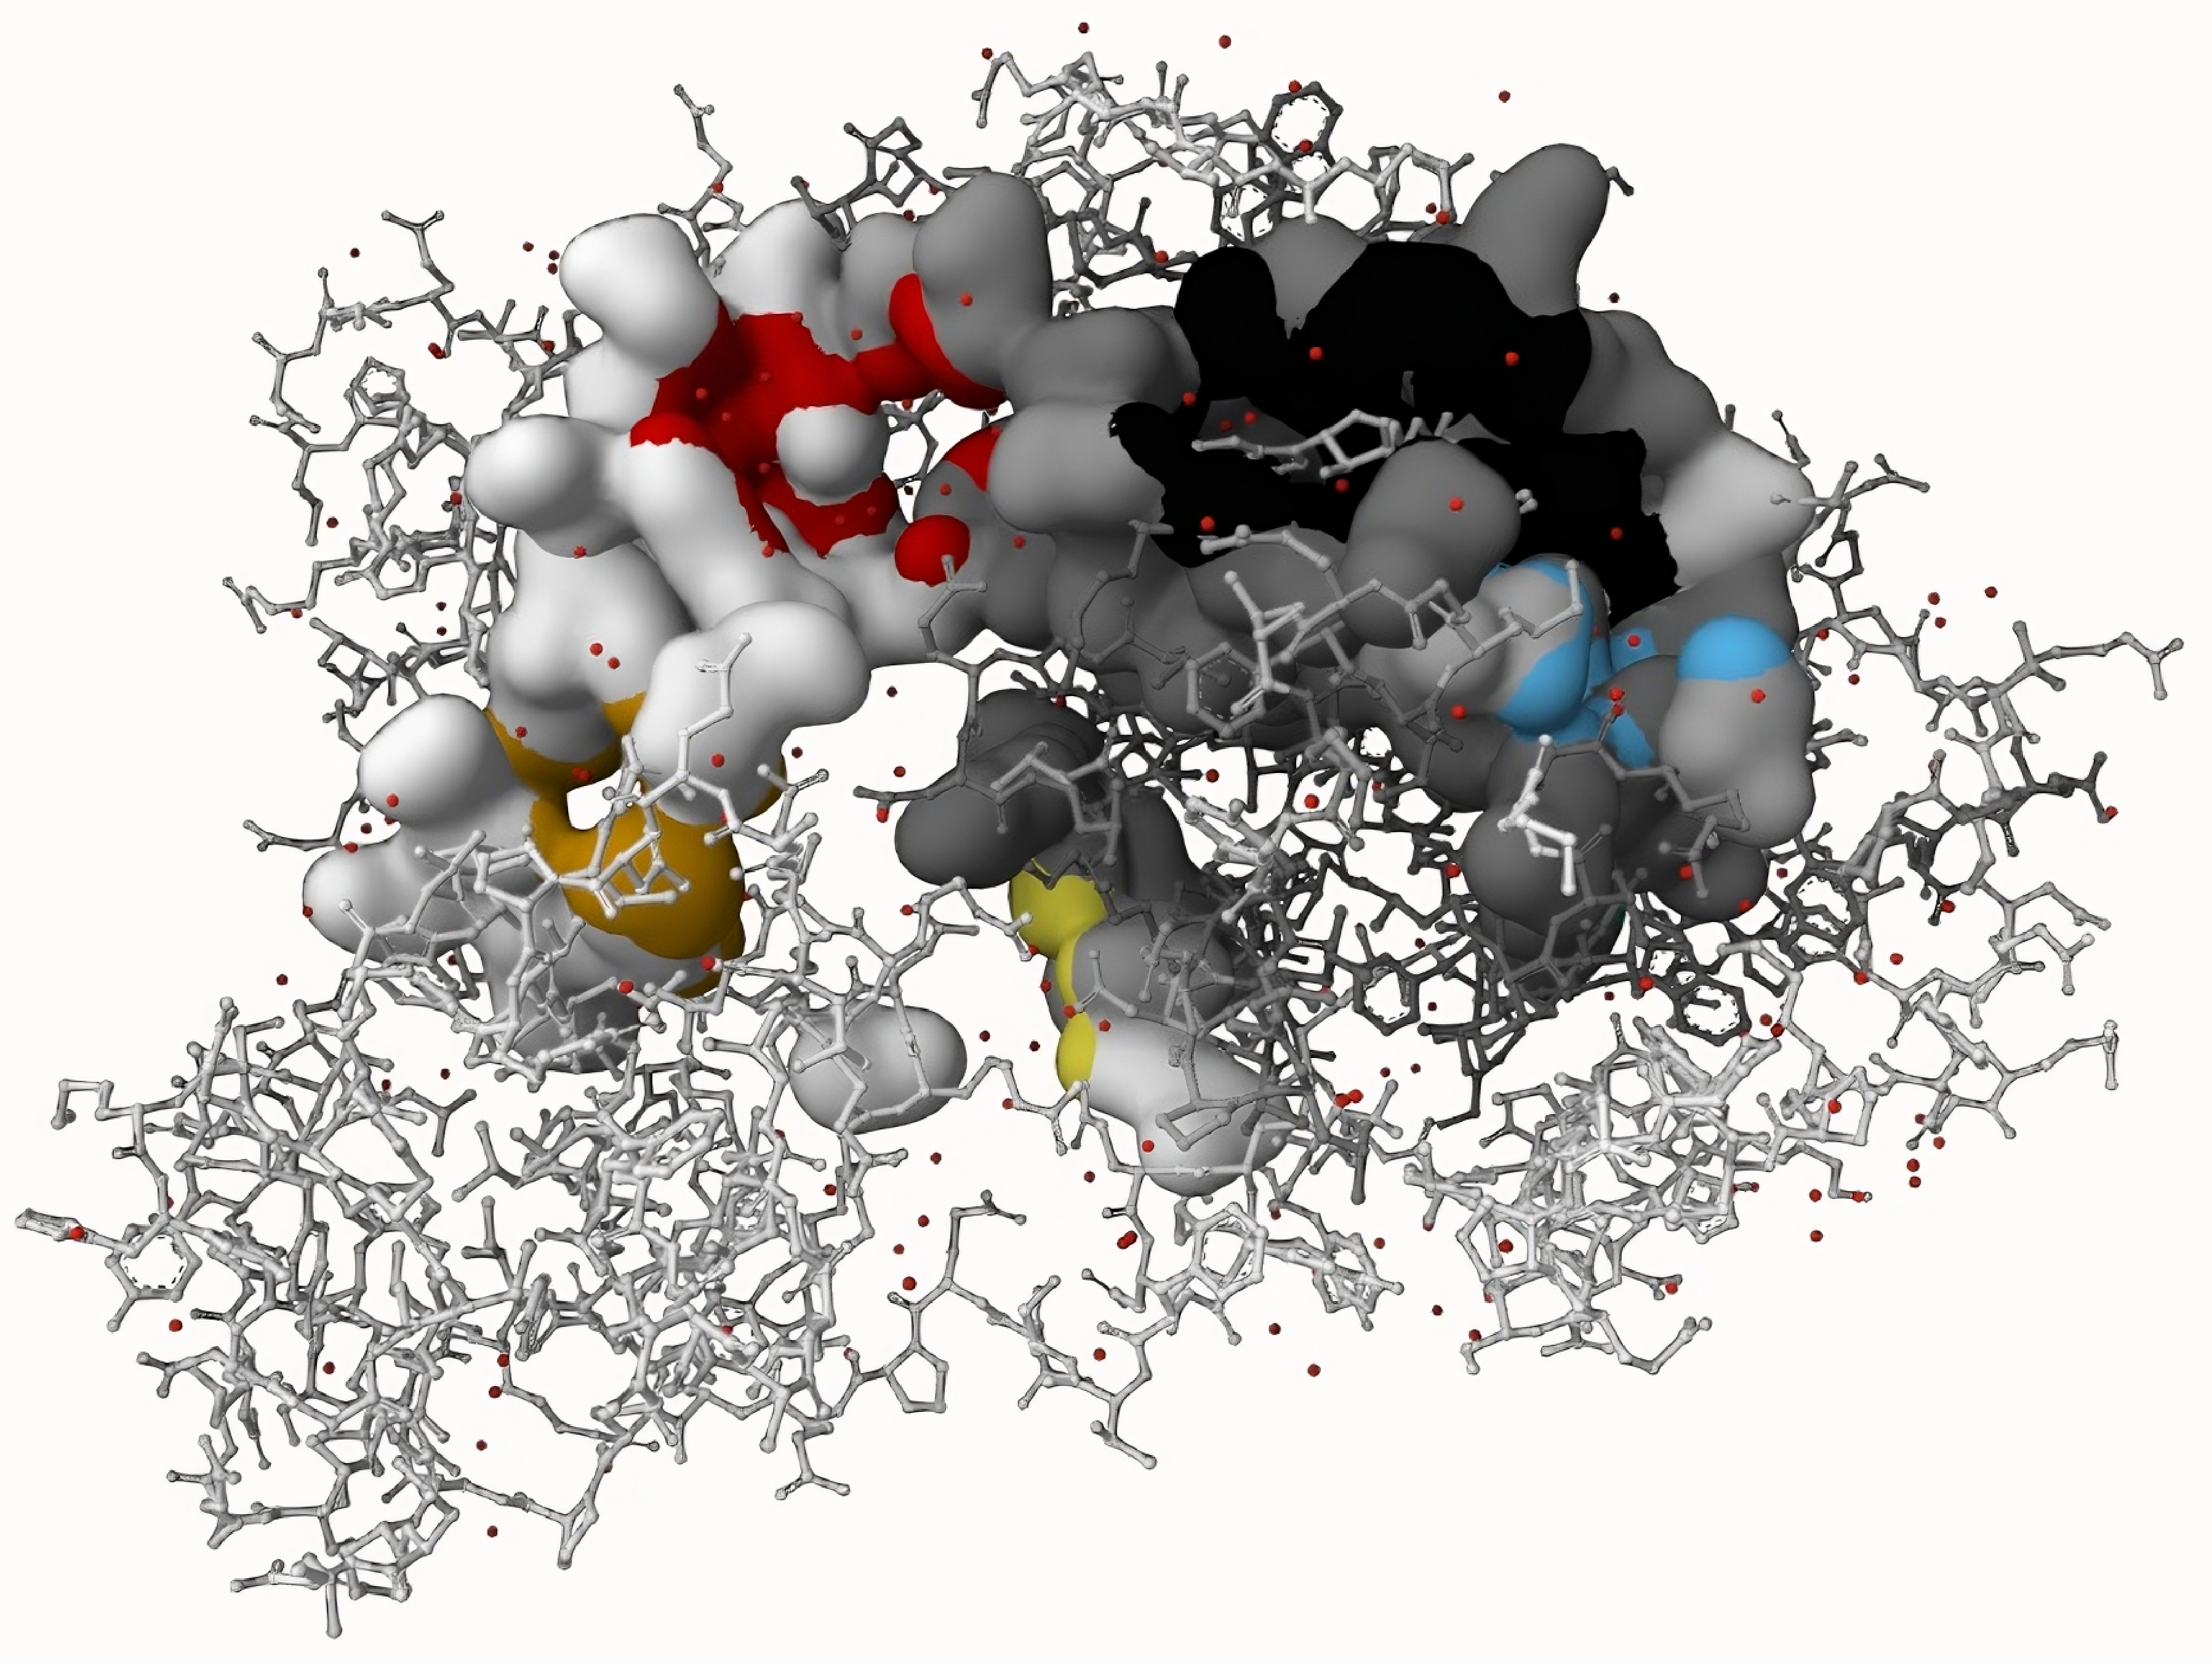
\includegraphics[width=0.8\linewidth]{img/molstar.pdf}
\end{center}

In the second picture, the 3D representation of the protein 2SRC is shown.
As the 3D viewer, we used the Mol* library, which is actively developed.
The viewer is interactive and there are plenty of options to customize the visualization.
In this picture, the ball-and-stick representation is used for the protein, the pockets are shown in the surface representation and each of the pockets is colored differently. Moreover, the atoms are colored by their conservation score in gray.

\end{posterbox}

\begin{posterbox}[column=1, name=result2, below=result1,
headerColorOne=violet!90!blue!60, boxColorOne=violet!15]{Backend plugins}

We have introduced a plugin system to PrankWeb. Newly created components allow the developers to create new plugins that can be used to postprocess the predicted binding sites. As an example of the plugin system, we implemented a plugin that allows molecular docking into the predicted binding sites.
The implementation may be integrated into the existing server architecture, so there are minimal changes to the existing codebase and deployment.

%TODO: add some pictures of the plugin or the example (docking)?
%\begin{center}
%\begin{tabular}{lrr}
% & \textbf{SomeProgram} & \textbf{ThisThesis} \\
%\hline
%Process A & 50\% & 58\% \\
%Time for A & 35 days & \textcolor{green!80!black}{35 seconds} \\
%Process B & \textcolor{red}{15\%} & 55\% \\
%Time for B & 1 day & 8 hours \\
%Price & 66.6 EUR & free
%\end{tabular}
%\end{center}
\end{posterbox}

%\begin{posterbox}[column=1, name=result3, below=result2, headerColorOne=green!50!yellow, boxColorOne=green!10]{Main result}
%\large\bfseries
%\vspace{1ex}
%\begin{center}
%Program ThesisProgram solves the problem better than OtherProgram if X, and faster if Y.
%\end{center}
%\vspace{.5ex}
%\end{posterbox}

\begin{posterbox}[column=1, name=conclusion, below=result2, bottomaligned=tech]{Source codes \& Contact}

%TODO: maybe add a QR code with the link to the repository or the running instance.

\begin{minipage}[t]{\linewidth}
	\begin{minipage}[t]{0.75\linewidth}
		Thesis supervisor: \textbf{doc. RNDr. David Hoksza, Ph.D.}, Department of Software Engineering\\

		GitHub repository (see the branches): \textbf{github.com/luk27official/prankweb}

		Running instance: \textbf{prankweb.cz}\\

		I'd also like to thank the CUSBG members.
		%TODO: use the cusbg or mine?
	\end{minipage}
	\quad
	\begin{minipage}[t]{0.20\linewidth}
		\vspace{-2ex}
		
\includegraphics[width=1\linewidth]{./img/qr_prankweb_cz.png} %TODO: use running instance or github?
		\begin{center}
			Try it out yourself!
		\end{center}
	\end{minipage}
\end{minipage}


\end{posterbox}

\end{poster}
\end{document}
